\chapter{Quantum Error Correction and Fault Tolerance}
\lecture{19}{20 Nov. 10:30}{}  % L18이랑 통합
\section{Introduction}
Quantum noise는 universal quantum computer를 설계하기 위해 가장 중요하게 다뤄져야 하는 요소이다. Chapter 3에서는 quantum error를 표현하는 방법을 배웠고 이제 이 챕터에서는 quantum error를 정정하는 방법을 소개하려고 한다.

\section{Some distance measure}
Quantum noise로 인해서 state가 얼마나 많이 달라졌는지를 평가하기 위해서, \textit{distance measure}를 정의해야 한다. 이를 위해서 먼저 classical information에 대한 distance measure를 소개하고 이를 quantum information에 대해서 확장한 distance measure를 소개한다.
\subsection{Distance measures for classical information}
동일한 random variable $X$에 대해, 서로 다른 두 probability distribution $\{p_x\}$와 $\{q_x\}$를 가정하자. 이 두 distribution의 차이를 나타내기 위해 사용할 수 있는 한 가지 방법은 \textit{total variation distance (TVD)}이다:
\begin{equation*}
    D(p, q) \triangleq \frac{1}{2} \sum_{x}|p_x-q_x|
\end{equation*}
만약 두 분포가 동일하다면, TVD는 0이 된다. 반대로 두 분포가 \textit{orthogonal}하다면, TVD는 1이된다.\\
Total variation distance는 다음과 같은 성질을 가진다.
\begin{itemize}
    \item Symmetry: $D(p, q)=D(q, p)$
    \item Non-negativity: $D(p, q) \geq 0$
    \item Triangle inequality: $D(p, q) \leq D(p, r)+D(r, q)$
\end{itemize}
\vspace{1em}
반면, \textit{fidelity}를 사용하여 두 분포의 차이를 나타낼 수도 있다.
\begin{equation*}
    F\left(p_x, q_x\right) \triangleq \sum_x \sqrt{p_x q_x} 
\end{equation*}
마찬가지로 두 분포가 동일하다면, fidelity는 1이 되고 반대로 두 분포가 \textit{orthogonal}하다면 fidelity는 0이 된다. Fidelity 역시 0과 1사이의 값을 가지며 TVD와 반비례하는 값을 가진다.

(\textit{operational meaning}) TVD는 sample space의 가능한 모든 subset $S$에 대해서 두 분포의 차이가 최대가 되게하는 $S$의 space에 대한 TVD와 동일한 값을 가진다.
\begin{equation*}
    D(p, q)=\max _S|p(S)-q(S)|=\max _S\left|\sum_{x \in S} p_x-\sum_{x \in S} q_x\right|,
\end{equation*}


\subsection{Trace distance}
Trace distance는 TVD를 quantum distance measure로 확장한 것이다.\footnote{quantum density matrix에서 대각성분은 확률을 의미 한다.} ($|A| \triangleq \sqrt{A^\dagger A}$)
\begin{equation*}
    D(\rho, \sigma) \equiv \frac{1}{2} \operatorname{Tr}[|\rho-\sigma|],
\end{equation*}
Trace distance가 가지는 중요한 성질중에 하나는 바로 unitary operation에 대해서 invariant하다는 것이다.
\begin{equation*}
    D(\rho, \sigma)=D(U\rho U^\dagger, U\sigma U^\dagger)
\end{equation*}
Trace distance는 다음과 같이 나타낼 수도 있으며, 이는 가능한 모든 POVM set에 대해서 두 trace의 차이가 최대가 되도록 하는 POVM에 대한 trace distance로 정의할 수 있음을 의미한다. (TVD의 두 번째 정의)
\begin{equation*}
    D(\rho, \sigma)=\max _{\left\{M_x\right\}}\left|\operatorname{Tr}\left[M_x \rho\right]-\operatorname{Tr}\left[M_x \sigma\right]\right|,
\end{equation*}
Trace distance에 대해 중요한 특징이 존재하는데 이는 동일한 trace preserving quantum operator를 가했을 때, trace distance는 \textit{증가할 수 없다}는 정리이다.
\begin{equation*}
    D(\mathcal{E}(\rho), \mathcal{E}(\sigma)) \leq D(\rho, \sigma) 
\end{equation*}

\subsection{Quantum fidelity} \label{sec:quantum-fidelity}
다음으로 살펴볼 Quantum fidelity는 fidelity를 quantum distance measure로 확장한 것이다.
\begin{equation*}
    F(\rho, \sigma) \triangleq \operatorname{Tr} \sqrt{\sqrt{\rho} \sigma \sqrt{\rho}}
\end{equation*}
Quantum fidelity는 trace distance와 유사하게 다음과 같은 성질을 가진다.
\begin{itemize}
    \item Symmetry: $F(\rho, \sigma)=F(\sigma, \rho)$
    \item Invariant of unitary: $F(\rho, \sigma)=F(U\rho U^\dagger, U\sigma U^\dagger)$
    \item Operation inequality: $F(\mathcal{E}(\rho), \mathcal{E}(\sigma)) \geq F(\rho, \sigma)$
\end{itemize}

만약, $\rho=\sum_i r_i|i\rangle\langle i|, \sigma=\sum_i s_i|i\rangle\langle i|$가 commute하다면 quantum fidelity는 classical fidelity와 같다.
\begin{equation*}
    F(\rho, \sigma)=\operatorname{Tr}\left[\sqrt{\sum_i r_i s_i|i\rangle\langle i|}\right]=\sum_i \sqrt{r_i s_i}=F\left(r_i, s_i\right)
\end{equation*}
또한, 만약 두 state중에서 적어도 하나가 pure state라면, quantum fidelity는 다음과 같이 나타낼 수 있다.\footnote{계산이 간단하다.}
\begin{equation*}
    F(|\psi\rangle, \rho)=\operatorname{Tr}[\sqrt{\langle\psi| \rho|\psi\rangle|\psi\rangle\langle\psi|}]=\sqrt{\langle\psi| \rho|\psi\rangle} .
\end{equation*}

Quantum fidelity의 중요한 정의는 Uhlmann's theorem에 의해 주어진다. 이 정리는 양자 상태 사이의 fidelity를 pure state들의 overlap으로 생각할 수 있음을 주장한다.
\begin{theorem}[Uhlmann's theorem]
    $\rho$와 $\sigma$가 quantum system $Q$의 state일 때, quantum system $Q$의 복사본인 다른 system $R$에 대해 다음이 만족한다.
    $$ F(\rho, \sigma)=\max _{|\psi\rangle,|\varphi\rangle}|\langle\psi | \varphi\rangle| $$
    $\ket \psi, \ket \varphi$는 $\rho$, $\sigma$에 대해 $RQ$로 purification하여 나타낸 가능한 모든 pure state이다.
\end{theorem}

Quantum fidelity는 가능한 모든 POVM에 대한 classical fidelity를 사용하여 정의할 수 있다.
\begin{equation*}
    F(\rho, \sigma)=\min_{\{\Pi_m\}} F\left(p_m, q_m\right)
\end{equation*}

마지막으로, trace distance와 fidelity는 다음과 같은 관계를 만족한다.
\begin{equation*}
    1-F(\rho, \sigma) \leq D(\rho, \sigma) \leq \sqrt{1-F(\rho, \sigma)^2} .
\end{equation*}

\section{The basic code and Shor code}
\subsection{Classical error correction}
\begin{figure}
    \centering
    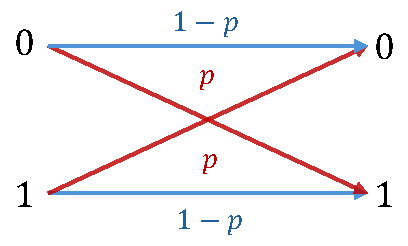
\includegraphics[width=0.3\textwidth]{figures/classical-bit-flip.pdf}
    \caption{Classical bit flip}
    \label{fig:bit-flip}
\end{figure}

Classical channel에서 발생할 수 있는 가장 간단한 오류인 bit flip error를 생각해보자. 아무런 인코딩도 하지 않는다면 수신자의 입장에서 bit 1을 받았을 때 원래 1인지 아니면 0이었는데 bit flip error가 발생한 것인지를 구분할 수 없다.
이를 해결하기 위해 $0$이나 $1$대신에 비트를 반복해서 $000$, $111$으로 인코딩하여 bit flip error를 해결할 수 있다. 만약 오류의 발생확률 $p$가 충분히 작다면 오류가 발생한 bit string이 $001$일 때 $000 \rightarrow 001$의 확률이 $111 \rightarrow 001$의 확률보다 작다는 사실을 이용하여 오류 정정을 할 수 있다. 

\textit{Repetition code}의 성공 확률은 오류가 발생하지 않을 확률과 하나의 단일 비트에만 오류가 발생했을 확률의 합이며,
\begin{equation*}
    (1-p)^3+3p(1-p)^2 = 1 + 2p^3 - 3p^2
\end{equation*}
실패 확률은 2개의 이상의 비트에 오류가 발생했을 확률이다.
\begin{equation*}
    P_e  = 3p^2(1-p) + p^3 = - 2p^3 + 3p^2 
\end{equation*}
그렇다면, 오류 확률 $p$가 얼마나 작을 때 오류 정정 코드를 사용하는 것이 유리한지를 오류 정정을 하지 않았을 때의 실패 확률 $p$와 비교하여 계산할 수 있다.
\begin{equation*}
    p_e = -2p^3 + 3p^2 < p \quad \rightarrow \quad p < \frac{1}{2}
\end{equation*}

\subsection{The three qubit bit flip code}
Classical communication에서 이미 검증된 repetition code를 quantum communication에 바로 적용할 수 없는 이유는 다음과 같다.
\begin{itemize}
    \item No cloning : 주어진 임의의 양자상태를 복사할 수 없으므로 repetition이 불가능하다.
    \item Continuous error : 양자 채널은 bit flip error말고도 다른 다양한 오류가 존재한다.
    \item Measurement : 오류 정정을 위해서 state를 확인하면 기존의 quantum state가 붕괴된다.
\end{itemize} 
지금부터는 이러한 문제들을 어떤 방식을 도입하여 해결하였는지 소개하려고 한다. 먼저, $\ket \psi$에 $p$의 확률로 $X$ gate가 작용하여 state가 $X \ket \psi$로 변하는 bit flip error에 대해서만 생각해보자.
이를 해결하기 위해서 $\ket{0_L}, \ket{1_L}$을 physical qubit 3개로 표현되는 logical qubit으로 인코딩하자. \footnote{두 state $\ket 0, \ket 1$은 서로 orthogonal state이므로 복사할 수 있다.}
\begin{equation*}
    a|0\rangle+b|1\rangle \rightarrow a|000\rangle+b|111\rangle \equiv a\left|0_L\right\rangle+b\left|1_L\right\rangle,
\end{equation*}

그러나, logical qubit을 사용하더라도 여전히 오류가 발생했는지 확인하기 위해서 중간에 상태를 관측하면 기존의 정보를 모두 잃어버리게 되므로 \textbf{state를 관측하지 않고도 오류의 발생을 감지할 수 있는} 다른 방법이 필요하다.
이를 위해서 \textit{Syndrome measurement}를 제안한다. 
\begin{itemize}
    \item $P_0 = |000\rangle\langle 000| + |111\rangle\langle 111|$ : 오류가 발생하지 않음
    \item $P_1 = |100\rangle\langle 100| + |011\rangle\langle 011|$ : 첫 번째 qubit에 bit flip이 발생함
    \item $P_2 = |010\rangle\langle 010| + |101\rangle\langle 101|$ : 두 번째 qubit에 bit flip이 발생함
    \item $P_3 = |001\rangle\langle 001| + |110\rangle\langle 110|$ : 세 번째 qubit에 bit flip이 발생함
\end{itemize}

이 syndrome measurement set을 사용하면, 발생할 수 있는 모든 오류\footnote{여기서는 single bit flip error만을 커버한다.}들의 subspace에 projection 시키기 때문에 측정 후에도 quantum state의 정보는 그대로 유지된다. 
\begin{equation*}
    \frac{P_0 \ket \psi}{\langle \psi | P_0^\dagger P_0 | \psi \rangle } = \frac{a|000\rangle + b |111\rangle}{a\langle 000|+ b\langle 111| ( |000\rangle\langle 000| + |111\rangle\langle 111| )a|000\rangle+b|111\rangle} = \frac{a|000\rangle + b|111\rangle}{a^2 + b^2} = \ket \psi
\end{equation*}
Syndrome measurement set을 사용해서 얻은 outcome을 확인하면, 어떤 qubit에 bit flip이 발생하였는지 알 수 있고 그 qubit에 $X$ gate를 가하여 오류를 정정할 수 있다. 

\vspace{1em}

Quantum repetition code의 실패 확률 역시 classical repetition code와 동일하게 $P_e = - 2p^3 + 3p^2$이며, $p < 1/2$일 때 오류 정정을 하지 않을 때보다 더 정확도가 증가한다. 그러나 quantum bit flip error는 classical bit flip error처럼 단순하게 실패 확률을 분석해서는 안된다.
예를 들어, 오류가 발생하기 전 상태가 $\ket +$였다면, bit flip error는 아무런 영향을 주지 못하기 때문이다. 따라서 \textit{state distance}의 관점에서 오류를 분석할 필요가 있다. (오류가 없는 이상적인 상태는 항상 pure state이므로 \textit{fidelity}를 $F = \sqrt{\langle \psi | \rho | \psi \rangle}$로 쉽게 계산할 수 있으므로 fidelity를 사용하자.)

Quantum error correction의 목표는 \hyperref[sec:quantum-fidelity]{fidelity}를 증가시키는 것이다.\footnote{두 상태가 유사할수록 fidelity가 증가한다.}  만약 오류 정정을 하지 않는다면, output state는 다음과 같이 표현된다.
\begin{equation*}
    \rho=(1-p)|\psi\rangle\langle\psi|+p X|\psi\rangle\langle\psi| X .
\end{equation*}
따라서 두 상태간의 fidelity는 다음과 같이 계산된다. 주어진 항에서 $\langle \psi | X | \psi \rangle$는 확률을 나타내는 값이므로 음수가 될 수 없다. $\ket \psi$가 computational state일 때, $\langle \psi | X | \psi \rangle = 0$이므로 minimum fidelity는 $\sqrt{1-p}$이라는 사실을 알 수 있다.
\begin{equation}
    F(\ket \psi \bra \psi, \rho)=\sqrt{\langle\psi| \rho|\psi\rangle}=\sqrt{(1-p)+p\langle\psi| X|\psi\rangle\langle\psi| X|\psi\rangle} \label{eq:fidelity-1}
\end{equation}
반면, 오류 정정을 수행했다면 1 bit flip error가 발생했더라도 오류정정을 통해 pure state를 그대로 유지할 수 있으므로 output state는 다음과 같고 
\begin{equation*}
    \rho_{QEC}=\left[(1-p)^3+3 p(1-p)^2\right]|\psi\rangle\langle\psi| + positive\ terms\ \cdots
\end{equation*}
fidelity는 다음의 lower bound를 가진다.
\begin{equation}
    F(\ket \psi \bra \psi, \rho_{QEC})  = \sqrt{(1-p)^3+3 p(1-p)^2 + positive\ terms\ \cdots}  \ge \sqrt{(1-p)^3+3 p(1-p)^2} \label{eq:fidelity-2}
\end{equation}
Eq.~\eqref{eq:fidelity-1}보다 Eq.~\eqref{eq:fidelity-2}의 값이 더 커지게 만들기 위해서는 $p < 1/2$여야 한다.

\vspace{1em}

Syndrome measurement를 이해하는 한 가지 다른 방법이 있다. 앞에서 제안한 4개의 projector를 사용하는 대신 2개의 observable을 측정한다고 생각해보자. 첫 번째로 $Z_1Z_2$\footnote{$Z_1Z_2 \triangleq  +\left((|00\rangle\langle 00|+|11\rangle\langle 11|)_{12} \otimes I_3\right) - \left((|01\rangle\langle 01|+|10\rangle\langle 10|)_{12} \otimes I_3 \right)$}를 측정하고
\begin{equation*}
    (Z_1Z_2) \qquad +1:(|00\rangle\langle 00|+|11\rangle\langle 11|)_{12} \otimes I_3, \quad-1:(|01\rangle\langle 01|+|10\rangle\langle 10|)_{12} \otimes I_3
\end{equation*}
이후 $Z_2Z_3$을 측정한다. 각각의 observable을 측정했을 때, $-1$이라는 outcome을 얻으면 해당 bit들의 값이 다르다는 것을 의미한다. 예를 들어 $Z_1Z_2$의 outcome이 $-1$이라면 첫 번째, 두 번째 qubit의 값이 다르다는 의미이다.
따라서 2개의 observable을 측정하여 얻은 outcome을 사용하여 어떤 qubit에 bit error가 발생하였는지를 추측하고 오류 정정을 수행할 수 있다. 


\begin{figure}[h]
    \begin{subfigure}[b]{0.5\textwidth}
        \centering
        \[
            \begin{array}{c}
            \Qcircuit @C=0.9em @R=1.6em {
                \lstick{\ket{\psi}} & \qw & \ctrl{1} & \ctrl{2} & \qw \\
                \lstick{\ket{0}} & \qw & \targ & \qw & \qw \\
                \lstick{\ket{0}} & \qw & \qw & \targ & \qw \\
            }
            \end{array}
            \]
        \caption{Three-qubit repetition code} \label{fig:repitition-circuit}
    \end{subfigure}
    \begin{subfigure}[b]{0.5\textwidth}
        \centering
        \[
            \begin{array}{c}
            \Qcircuit @C=1.0em @R=1.4em {
                \lstick{\ket{\psi}} & \qw & \ctrl{1} & \ctrl{2} & \gate{H} & \qw \\
                \lstick{\ket{0}} & \qw & \targ & \qw & \gate{H} & \qw \\
                \lstick{\ket{0}} & \qw & \qw & \targ & \gate{H} & \qw \\
            }
            \end{array}
            \]
        \caption{Three-qubit phase flip code} \label{fig:phse-flip-circuit}
    \end{subfigure}
    \caption{Three-qubit encoding circuits}
\end{figure}


\subsection{The three qubit phase flip code}
이번에는 phase flip error; $Z$ error에 대해 생각해보자. $Z$ error의 정정 역시 $X$ error의 정정과 동일한 방식을 도입하여 해결할 수 있다. Computational basis(X-basis) 대신에 Z-basis를 사용하여 state를 인코딩하며 syndrome measurement set을 사용하여 오류를 감지하고 오류가 발생한 qubit에 $Z$ gate를 가함으로서 phase flip error를 쉽게 해결할 수 있다. 
\begin{equation*}
    \left|0_L\right\rangle \equiv|+++\rangle, \quad\left|1_L\right\rangle \equiv|---\rangle .
\end{equation*}

\subsection{The Shor code}
지금까지 소개한 방식은 특정한 type의 single-qubit error만 해결할 수 있는 방법이다. 그렇다면, 다양한 single qubit error를 한번에 정정할 수 있는 방법은 없을까? Shor code가 바로 \textit{arbitrary single qubit error}를 모두 정정할 수 있는 방법이다. Shor code는 three qubit phase flip code와 bit flip code를 함께 적용한 간단한 방식을 사용한다.
\begin{enumerate}
    \item Encode the qubit using \textit{phase flip code}:
    \begin{equation*}
        |0\rangle \rightarrow|+++\rangle, \quad|1\rangle \rightarrow|---\rangle
    \end{equation*}
    \item Encoding each of the qubits \textit{bit flip code}:
    \begin{equation*}
        |+ \rangle = \frac{\ket 0 + \ket 1}{\sqrt 2} \rightarrow \frac{\ket{000} + \ket{111}}{\sqrt 2}, \quad |-\rangle = \frac{\ket 0 - \ket 1}{\sqrt 2} \rightarrow \frac{\ket{000} - \ket{111}}{\sqrt 2}
    \end{equation*}
\end{enumerate}
따라서 위의 인코딩 과정을 거치면 1개의 logical qubit은 \textbf{9개}의 physical qubit으로 구현된다. 
\begin{align*}
    |0\rangle \rightarrow\left|0_L\right\rangle & \triangleq \frac{(|000\rangle+|111\rangle)(|000\rangle+|111\rangle)(|000\rangle+|111\rangle)}{2 \sqrt{2}} \\
    |1\rangle \rightarrow\left|1_L\right\rangle & \triangleq \frac{(|000\rangle-|111\rangle)(|000\rangle-|111\rangle)(|000\rangle-|111\rangle)}{2 \sqrt{2}}
\end{align*}

이제 Shor code가 어뗳게 single qubit error를 정정할 수 있는지 살펴보자. 만약 $q_1$에 bit flip error가 발생했다면 observable $Z_1Z_2, Z_2Z_3$의 측정 결과로부터 $q_1$에 오류가 발생했다는 것을 알 수 있고 $X$ gate를 가하여 오류를 해결할 수 있다. 이처럼 Shor code는 bit flip error를 해결할 수 있다.
다음으로 $q_1$에 phase flip error가 발생했다고 하자. Phase flip은 computational basis에 대해서 qubit의 부호를 반전시키므로 $\ket{000} + \ket{111}$이었던 첫 번째 블록이 $\ket{000} - \ket{111}$으로 바뀌게 된다. 이 오류를 감지하기 위해서 우리는 각 블록($\ket{q_1q_2q_3}$)의 부호를 비교할 수 있도록 syndrome measurement를 사용할 수 있다. 
측정 결과로 첫 번째 블록과 두 번째 블록의 부호가 다르고 두 번째 블록과 세 번째 블록의 부호가 동일하다는 정보를 알게 되면, 첫 번째 블록 안의 어떤 qubit에서 phase flip이 발생했다고 추정할 수 있기 때문에 첫 번째 블록에 속한 qubit에 $Z$ gate를 가하여 phase flip error도 해결할 수 있다. Phase flip error를 감지하기 위해 사용하는 syndrome measurement는 다음과 같다.
\begin{equation*}
    X_1X_2X_3X_4X_5X_6, \quad X_4X_5X_6X_7X_8X_9
\end{equation*}
그렇다면 $q_1$에 bit flip error와 phase flip error가 동시에 발생했을 때는 어떻게 될까? 이 경우에는 단순히 bit flip error를 정정하는 단계와 phase flip error를 정정하는 단계를 모두 수행하여 문제를 해결할 수 있다.

이제 마지막으로, Shor code가 \textit{arbitrary single qubit error}를 정정할 수 있음을 보이고자 한다. 흥미롭게도, arbitrary single qubit error를 정정하는 과정 또한, 앞에서 설명했던 bit flip error와 phase flip error를 정정하는 두 방법을 적용하는 것으로 쉽게 해결할 수 있다.
이는 단일 큐빗에서 발생할 수 있는 \textbf{연속적인} 오류를 정해진 discrete subset of errors (i.e., X, Z, XZ)을 정정함으로써 모두 해결할 수 있다는 것을 의미한다.
이것이 왜 가능한 걸까? 첫 번째 qubit에 arbitrary single qubit error가 발생했다고 하자. 이 오류는 Kraus operator $\{E_i\}$를 사용하여 다음과 같이 표현될 수 있다.
\begin{equation*}
    \mathcal{E}(|\psi\rangle\langle\psi|)=\sum_i E_i|\psi\rangle\langle\psi| E_i^{\dagger}
\end{equation*}
전체 오류 대신, 합의 각 항 $E_i | \psi \rangle \langle \psi | E_i^\dagger$에 대한 정정을 생각해보자. 
우리는 어떤 single qubit operator도 다음과 같이 Pauli operator의 linear combination으로 표현할 수 있다는 사실을 알고있다.\footnote{$Y= XZ$}
\begin{equation*}
    E_i = e_{i0} I + e_{i1} X_1 + e_{i2} Z_1 + e_{i3} X_1Z_1
\end{equation*}
따라서 이 operator가 pure state $\ket \psi$에 작용한다면, 다음 4개의 항의 superposition 상태가 될 것이다.
\begin{equation*}
    |\psi\rangle, \quad X_1|\psi\rangle, \quad Z_1|\psi\rangle, \quad X_1 Z_1|\psi\rangle 
\end{equation*}
Shor code에서 사용하는 syndrome measurement는 $I, X, Z, XZ$가 가해졌을 때 얻을 수 있는 error들의 subspace로 \textit{projection}시키는 역할을 수행하기 때문에, syndrome measurement를 가하면 error state들의 superposition state가 붕괴해서 하나의 state가 된다.
각각의 상태는 Shor code의 오류 정정 과정을 사용할 수 있으므로(apply X, Z, XZ), 최종적으로 오류가 정정된 state로 변하게 된다. 
이것이 바로 Shor code가 arbitrary single qubit error를 정정할 수 있는 이유이다.

\begin{figure}[h]
    \centering
    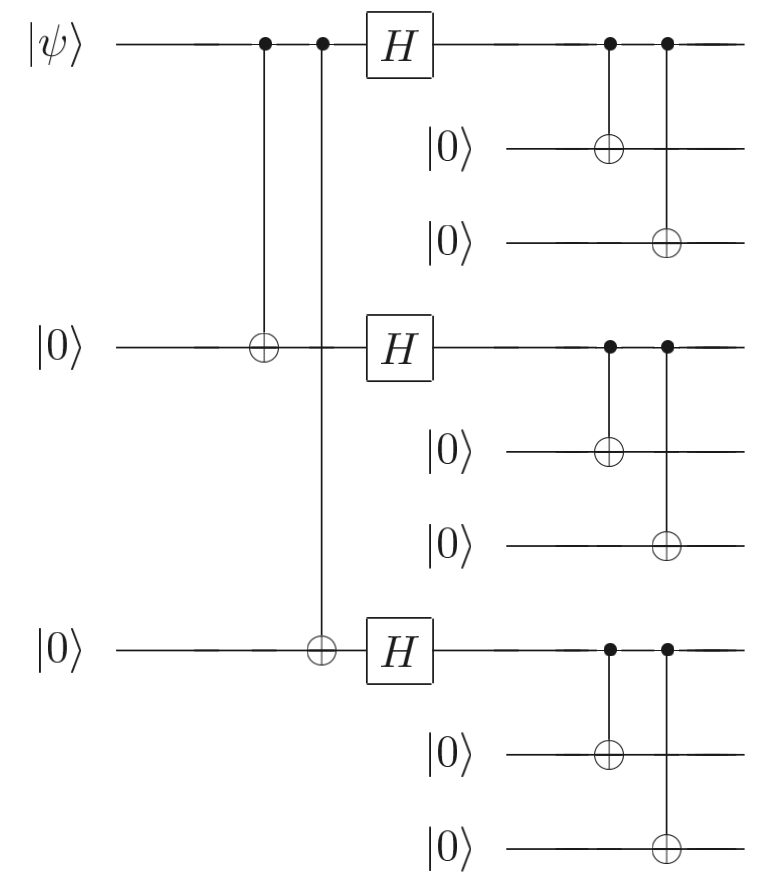
\includegraphics[width=0.4\textwidth]{figures/Shor_code.png}
    \caption{Shor code circuit} \label{fig:Shor-circuit}
\end{figure}

\lecture{20}{25 Nov. 10:30}{}
\section{Theory of QEC}

\subsection{QEC conditions}

\subsection{Discretization of the errors}

\subsection{Independent error models}

\subsection{Degenerate codes}


\section{Constructing quantum codes}
\subsection{Classical linear codes}


\lecture{21}{1 Dec. 10:30}{}
